\documentclass{standalone}
\usepackage[utf8]{inputenc}
\usepackage{amsmath}
\usepackage{amssymb}

\usepackage{tikz}
\usetikzlibrary{shapes.geometric, arrows}

\tikzstyle{startstop} = [rectangle, rounded corners, minimum width=3cm, minimum height=1cm,text centered, draw=black, fill=red!30]
\tikzstyle{io} = [trapezium, trapezium left angle=70, trapezium right angle=110, minimum width=3cm, minimum height=1cm, text centered, draw=black, fill=blue!30]
\tikzstyle{process} = [rectangle, minimum width=3cm, minimum height=1cm, text centered, draw=black, fill=orange!30]
\tikzstyle{decision} = [diamond, minimum width=3cm, minimum height=1cm, text centered, draw=black, fill=green!30]
\tikzstyle{arrow} = [thick,->,>=stealth]
\tikzstyle{fdot} = [circle, minimum width=4pt, fill]
\tikzstyle{line} = [thick,>=stealth]

\begin{document}

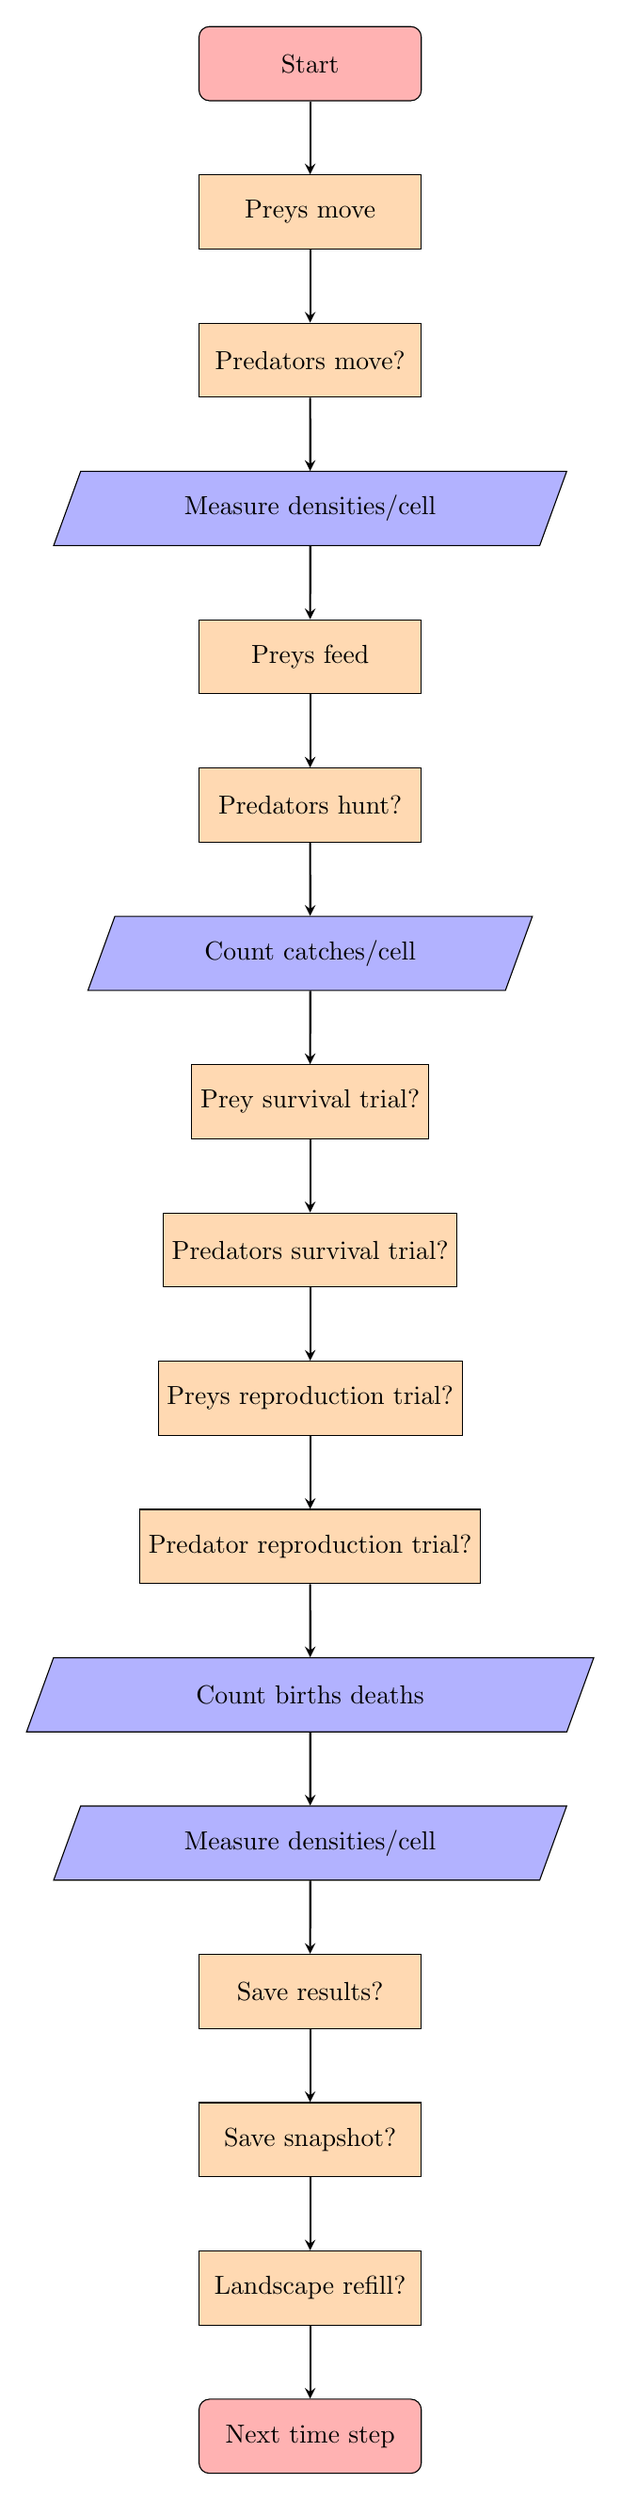
\begin{tikzpicture}[node distance=2cm]

\node (start) [startstop] {Start};
\node (pro1) [process, below of=start] {Preys move};
\node (dec1) [process, below of=pro1] {Predators move?};
%\node (pro2) [process,  right of=dec1, xshift=2.5cm] {Predotors move};
\node (io1) [io, below of=dec1] {Measure densities/cell};
\node (pro3) [process, below of=io1] {Preys feed};
\node (dec2) [process, below of=pro3] {Predators hunt?};
%\node (pro4) [process,  right of=dec2, xshift=2.5cm] {Predotors hunt};
\node (io2) [io, below of=dec2] {Count catches/cell};
\node (dec3) [process, below of=io2] {Prey survival trial?};
%\node (pro5) [process,  right of=dec3, xshift=2.5cm] {Preys survival trial};
\node (dec4) [process, below of=dec3] {Predators survival trial?};
%\node (fdot1) [fdot, below of=dec4] {};
%\node (pro6) [process,  right of=dec4, xshift=2.5cm] {Predator survival trial};
%\node (fdot2) [fdot, below of=dec3, yshift=-3cm] {};
\node (dec5) [process, below of=dec4] {Preys reproduction trial?};
%\node (pro7) [process,  right of=dec5, xshift=2.5cm] {Preys reproduction trial};
%\node (dec6) [decision, below of=pro7] {Predators introduced?};
%\node (fdot3) [fdot, below of=dec6] {};
\node (pro8) [process,  below of=dec5] {Predator reproduction trial?};
%\node (fdot4) [fdot, below of=dec5, yshift=-3cm] {};
\node (io3) [io, below of=pro8] {Count births deaths};
\node (io4) [io, below of=io3] {Measure densities/cell};
\node (dec8) [process, below of=io4] {Save results?};
%\node (pro10) [process, right of=dec8, xshift=2.5cm] {Save results};
%\node (fdot6) [fdot, below of=dec8, yshift=1cm] {};
\node (dec9) [process, below of=dec8] {Save snapshot?};
%\node (pro11) [process, right of=dec9, xshift=2.5cm] {Save snapshot};
%\node (fdot7) [fdot, below of=dec9, yshift=0.5cm] {};
\node (dec7) [process, below of=dec9] {Landscape refill?};
%\node (pro9) [process,  right of=dec7, xshift=2.5cm] {Landscape refill};
%\node (fdot5) [fdot, below of=dec7, yshift=1.5cm] {};
\node (stop) [startstop, below of=dec7] {Next time step};

\draw [arrow] (start) -- (pro1);
\draw [arrow] (pro1) -- (dec1);
\draw [arrow] (dec1) -- (io1);
\draw [arrow] (io1) -- (pro3);
\draw [arrow] (pro3) -- (dec2);
\draw [arrow] (dec2) -- (io2);
\draw [arrow] (io2) -- (dec3);
\draw [arrow] (dec3) -- (dec4);
\draw [arrow] (dec4) -- (dec5);
\draw [arrow] (dec5) -- (pro8);
\draw [arrow] (pro8) -- (io3);
\draw [arrow] (io3) -- (io4);
\draw [arrow] (io4) -- (dec8);
\draw [arrow] (dec8) -- (dec9);
\draw [arrow] (dec9) -- (dec7);
\draw [arrow] (dec7) -- (stop);

\end{tikzpicture}

\end{document}